	
\documentclass[12pt]{article}
\usepackage{geometry} % see geometry.pdf on how to lay out the page. There's lots.
\geometry{a4paper} % or letter or a5paper or ... etc
% \geometry{landscape} % rotated page geometry
\usepackage{url}
\usepackage{graphicx}
\usepackage{multirow}
\usepackage[ruled,noend]{algorithm2e}
\usepackage[noend]{algorithmic}

\newcommand{\code}[1]{{\fontfamily{phv}\selectfont \small{\begin{tabbing} #1 \end{tabbing}}}}

\title{Natural Language Programming Analysis in Scala}
\author{\\ \'Eric Zbinden \\ \texttt{eric.zbinden@epfl.ch} \\ \\ Supervisors: \\Philippe Sutter(\texttt{philippe.sutter@epfl.ch})\\ Philipp Haller(\texttt{philipp.haller@epfl.ch})\\Prof. Viktor Kuncak(\texttt{viktor.kuncak@epfl.ch}) \\ \\ EPFL\\ Laboratory for Automated Reasoning and Analysis (LARA) \\ \url{http://lara.epfl.ch/}\\ Programming Methods Laboratory (LAMP) \\ \url{http://lamp.epfl.ch/} }
\date{\today}

\begin{document}

\maketitle
\newpage
\tableofcontents
\newpage

\section{Introduction}
...\\
For Java this was done by  

\section {Project Overview}
The main idea of this project is to apply an analysis similar to H{\o}st and {\O}stvold~\cite{DebugMN} but to Scala. Scala contains possibilities that JAVA don't contains; functional programming, local import. So I tried to focus on theses particularities as much as possible.

\section {Implementation}
The first thing is to retrieve information about a code. The best way is to create a plug-in for the Scala compiler. 

\subsection{Compiler plug-in}
My plug-in, named Scala-names, is inserted into the compiler phases right after phase 7:~\textit{refchecks}. It use the abstract syntax tree produced in previous phases to extract all objects named by the programmer. It could be variables names, objects names, methods names, parameters names or types names.\\

By lack of time, the analysis is run only on method names. But the plug-in could easily be improved to also analyze other objects.
The plug-in then check for every method definition found if that method have a given list of features. See~\ref{fs} for more details on features. Then the plug-in output for every method a list of "1" or "0" depending on this method satisfy or not a feature and the method name with source and position.

\subsection{Features}
\label{fs}
A feature is a boolean property that a method may satisfy or not. 

\begin{enumerate}
\item Return type is a collection :\\
	The return type is a collection. To be enough general to match a return of a List, a Set or a Map, it's implemented to match any class that extends the Traversable trait~\cite{travers}.
\item Return type is an Object : \\
	This feature match any return type that extends the AnyRef class~\cite{anyRef}.
\item Return type is Unit :\\
	This feature match if the return type is Unit.
\item Return type is boolean : \label{fBool}\\
	Straight forward, this feature match boolean return type.
\item Return type is an Integer :\label{fInt}\\
	Same as feature~\ref{fBool} with Integer return type.
\item Return type is a String : \\
	Same as features~\ref{fBool} and~\ref{fInt} with String return type.
\item Method take no parameter :\label{fNoParam}\\
	This method is a variant of feature~\ref{fNoParenthesis} .
\item Method is declared without parenthesis :\label{fNoParenthesis}\\
	%This feature is a variant of feature~\ref{fNoParam}.
In Scala when a programmer declare a function that take no argument, it's possible to write with or without parenthesis. With parenthesis indicate that this function have side effect; modifying data, printing out on std. In the AbstractSyntaxTree produced by the compiler, the parameters of a method are returned as a List of List. If the first list is empty, then it indicate that this method is declared without parameters and no parenthesis and should therefore have no side-effect. If the first list is of size one and contains an empty list, we have here a method declared without parameters but with parenthesis and thus with possible side-effect. And if the first list have a bigger size than one, it indicate we are dealing with a currified function.
\item Method body contains IF statement :\\
	The method body contain an IF branch. Note that the Scala compiler translate WHILE block and DO-WHILE block with a IF branch. These two case should not match this feature as the programmer did not write any IF branch. IF guard statement in pattern matching are not taken in account as IF branch. However an IF branch inside a pattern matching right hand side will match.\\
IF branch matching inside pattern matching right hand side:
\code{
ls \=match \{\\
\>case Nil =$>$\ false\\
\>case x\ ::\ xs =$>$\ if(x==0) true else false\\
\}
}
IF guard in pattern matching
\code{
ls \=match \{\\
\>case Nil =$>$\ false\\
\>case x\ ::\ xs if(x==0) =$>$\ true\\
\>case x\ ::\ xs =$>$ false\\
\}
}
\item Method body contains WHILE statement :\\
	The method body contains a WHILE statement. DO-WHILE statement are also considered as WHILE statement.
\item Method body contains TRY-CATCH statement :\\
	The method body contains a TRY-CATCH block. If a method body contains only the TRY block, it will also match.
\item Method body contains pattern matching : \\
	The method body contains pattern matching. If match if the method body contains a MATCH statement.
\item Method body contains explicit THROW statement :\\
	The method body contains a THROW statement. It match only if it's explicitly declared. A NumberFormatException raised by a wrong string applied to \textit{.toInt} will not match.
\item Method is currified : \\
	This feature is a variant of feature~\ref{fNoParenthesis}.
\item Method is self-recursive : \\
	This method call it-self in it's body. The feature don't match for other method even with surcharged identifiers.
\item Method name is a verb : \label{fVerb}\\
	This feature match if the method name is a verb. It could be an infinitive or a conjugated form. For this feature, it use the WordNet 2.1 database~\cite{wordNet} to determine it.
\item Method name is a noun :\\
	This feature match is the method name is a noun. As in feature~\ref{fVerb}, it use also the WordNet 2.1 database~\cite{wordNet}.
\item Method name is a camel case phrase : \label{fCamel}\\
	An unique word is not always meaningful to name a method. As C convention use underscore-separated words like "end\_of\_file", Java and Scala convention use camel case. Camel case is a practice of writing several words composed without white space but with the first letter of each word in uppercase. The first letter of the first word may or not be in uppercase.\\
This feature split the method name by the non-letter characters and by uppercase letters. Then it reconstruct potential acronym like in~\ref{fAcronym}. Then the feature will match if the split is composed at least of two words and if the second and followings words begin with an uppercase letter. Example:
\code{aCamel++Case\_PhraseWithXML \= =$>$ List(a, Camel, Case, Phrase, With, X, M, L)\\
\>=$>$ List(a, Camel, Case, Phrase, With, XML)\\
\>=$>$ true
}
Note that \textit{an\_Underscore\_Separated\_Phrase} will match this feature as all words, except the first, begin with an uppercase letter.
\item Method name contains an acronym :\label{fAcronym}\\
	An acronym is defined by the aggregation of uppercase letter and digit. It must start with a letter. Non-letter nor digit characters are considered, as in feature~\ref{fCamel}, as blank and thus discarded. Inside a camel case phrase, the acronym is construct correctly: the acronym inside \textit{XMLAsString} is reconstruct as \textit{XML}. But as the underscore will also considered as a blank, two acronym separated by an underscore will create one acronym instead of two.\\
This feature will match if the method name contains at least one word that is an acronym.
\item Method name match an abstract phrase construction : \\

\item Method name contains \textit{is} pattern :\label{fContainsIs}\\
	This feature match if the method name contains the word \textit{is}. \textit{is} can be written \textit{is} or \textit{Is}. As in features~\ref{fCamel} and~\ref{fAcronym}, the method name is split into words. Then if at least one word is \textit{is}, then the feature will match. 
\item Method name contains \textit{get} pattern :\label{fContainsGet}\\
	Straight forward, it's implemented the same way as feature~\ref{fContainsIs}.
\item Method name contains \textit{set} pattern :\label{fContainsSet}\\
	Same as features~\ref{fContainsIs} and~\ref{fContainsGet}.
\item Method name contains \textit{contains} pattern :\\
	Same as features~\ref{fContainsIs},~\ref{fContainsGet} and~\ref{fContainsSet}.
\item Method name is a valid JAVA name :\\
	A valid JAVA method name is a series of JAVA letters or JAVA digit that begin with a JAVA letter~\cite{jls_ident} and that is not a JAVA keyword~\cite{jls_keyword}. %pas tout à fait...

\item Method name is an operator :\\
	An operator is defined as a following of characters that are neither a letter neither a digit.
\item Method return type is completely contained into the method name :
\item Method return type is partially contained into the method name :\label{fReturnTypeComplete}\\
	This feature is a variant of feature~\ref{fReturnTypeComplete}. For composed type name, as programmer are often lazy, they often write it partially. One would by example write only "Tree" instead of "AbstractSyntaxTree". This feature will match in such case as previous feature will not. It will also match if the type is completely contained, like~\ref{fReturnTypeComplete}.
\item Method is right associative :\\
	Scala language is left associative. But a method name that finish with the \textit{:} character is right associative.
%ajouter qqch ici
\code{
1\ ::\ List(2, 3) \==$>$ List(2, 3)::.(1)\\
\>=$>$ List(1, 2, 3)
}
This feature match if the last character of the method name is \textit{:}\ .
\item Method is declared into another method :\label{fInner}\\
	Scala language permit declaration of functions inside function. It's a good way to declare subroutine that should not be used outside of this function.\\
This feature match if the method body contains a method declaration.
\item Method body contains inner method definition :\\
	This feature is the opposite of feature~\ref{fInner} and match if the method body contains a method declaration.
\item Method is overriding another method : \\
	This feature match if this method override another method.
\item Method is abstract :\\
	This feature match if the method body is empty.
\item Method is public :\\
	This feature match if this method is public. Note that inner function are always public but can't be accessed from outside.
\item Method is static :\\
	This feature match if this method is static. 
\item Method name finish with "s" :\label{fs}\\
	The last character of the method name is \textit{s}.
\item Method name finish with "ss" : \label{fss} \\
	This two lasts characters of the method name are both \textit{s}.

\end{enumerate}

\subsection{Clustering}
\label{cluster}
With the output of the Scala-names plug-in, I filled the \textit{k}-means algorithm~\cite{kMeans} hoping the result will be interesting. The implementation of the algorithm follow~\cite{kMeans} description with a random partition. K-means is sensible to the initial partitioning and its output may be different. The output may also contains empty clusters. As k-means reach a stable point fast, It's generally recommended to run several time the algorithm to be sure to obtain a fine result.\\
First question, how many cluster should we use ? A too small number of clusters will aggregate different groups of methods and a too high number of clusters will separate methods in a same group. I think the answer to this question really depend on the data set and what we want to find. See~\ref{cluster:exp} for answer based on this project.\\
At the end of the algorithm, we obtain clustered data. Fine, but the center of cluster is a raw position, as it's the average position of all its members. To obtain a position more readable an more meaningful, I discrete the position of the clusters depending on a threshold to obtain a position only composed of: $0$, $1$ or $?$. If for a given dimension the value is lower than the threshold, the value is lowered to $0$. Respectively if the value is higher than $1-threshold$, the value is raised to $1$. And if the value is higher than the threshold and lower than $1-threshold$ the value is set to undefined: $?$. See figure~\ref{discrete} for an example on two dimensions.\\
Then I do one more step of k-means to check the effect of the discretization to the clusters. Here another question is raised: what's a relevant threshold ? It should be small enough to be as most correct but big enough to have a minimum of undefined values. See the respond in section~\ref{threshold}.
\begin{figure}[tbc]
\centering
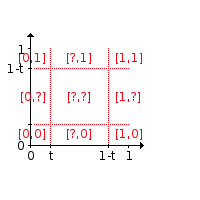
\includegraphics[width=5cm]{discrete.png}
\caption{Discretization of a cluster of two dimensions}
\label{discrete}
\end{figure}

\section {Experimental Results}

\subsection {Clustering}
\label{cluster:exp}
To answers the two questions of section~\ref{cluster}, I ran 100 times the k-means algorithm on the output of the Scala-names plug-in of the Scala library with different numbers of clusters. I took five mean metrics with confidence interval of 95\%: the number of empty clusters, the number of undefined values in all clusters, the average distance of methods to their respective cluster, the cluster average size and the error due to discretization modeled by the number of methods moving after a one-step check. 
\subsubsection{Number of clusters}
For this series of experiments, the threshold was fixed at 0.15 . 
\\ \\
\begin{center}
\begin{tabular}{c c}
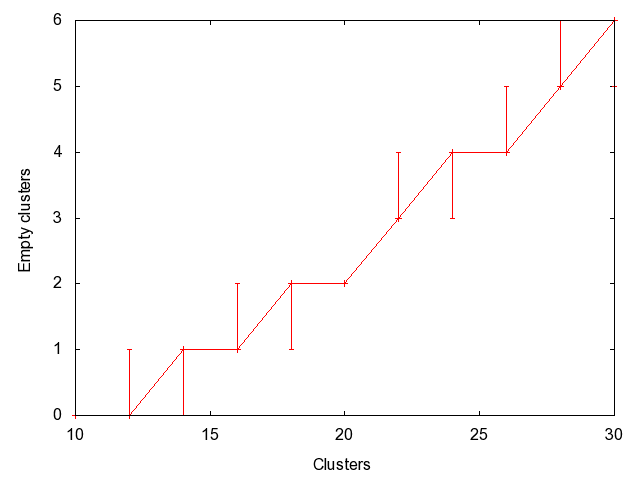
\includegraphics[width=5cm]{emptyCluster.png}
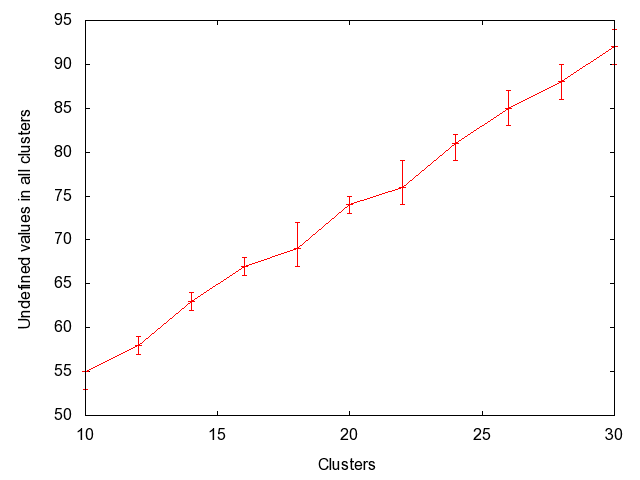
\includegraphics[width=5cm]{questionMark.png}
\end{tabular}\\
\begin{tabular}{c c c}
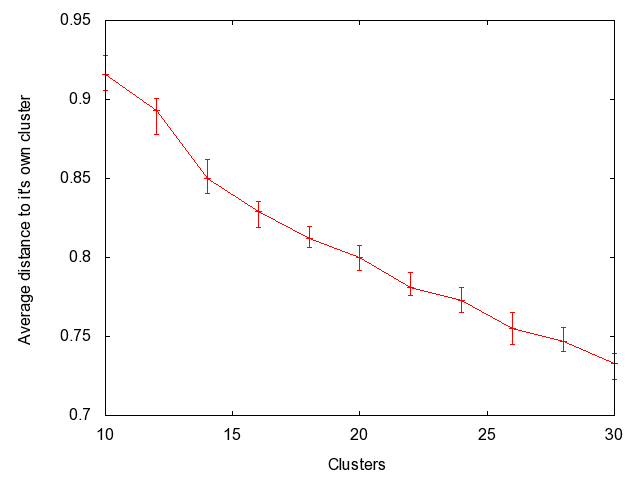
\includegraphics[width=5cm]{averageDist.png}
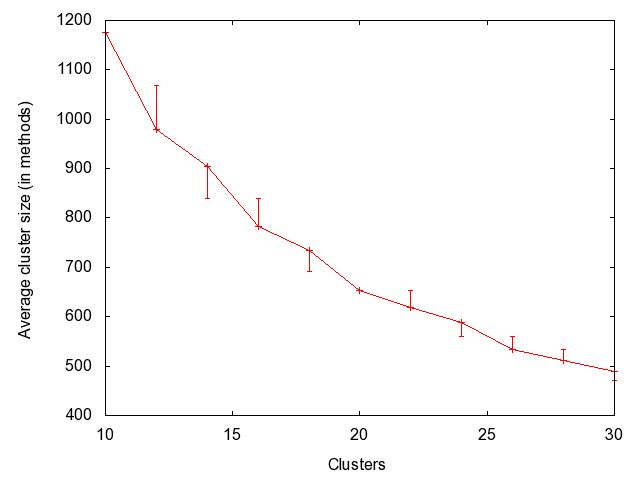
\includegraphics[width=5cm]{averageClusterSize.png}
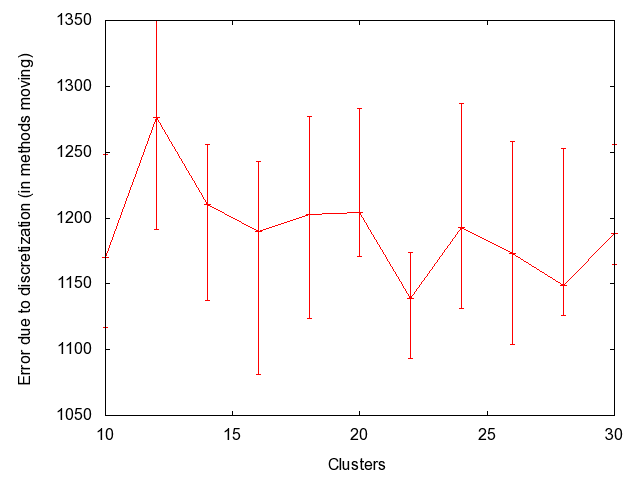
\includegraphics[width=5cm]{switched.png} %REFAIRE le graphic 5 pour l'ortho
\end{tabular}
\end{center}

\begin{enumerate}
\item As the number of clusters increase, the number of empty clusters increase too. With 30 clusters we reach 6 empty clusters. It represent a percentage of empty cluster of 20\%, which is pretty high. As The computational time of the algorithm also increase with a higher number of cluster, it suggest that a lower number of clusters is better.
\item To be independent of the first metric, the second it is calculated only with non-empty cluster. The number of undefined values in the clusters also increase with the cluster number on a basis of $\frac{2}{3}$. This is bad as we can't deduce anything from them.
\item The third metric seams not really relevant. If the distance of a method to it's own cluster decrease, that's good, as the cluster is a better representation of its members. But as the result for ten cluster is already below a distance of one, a so small difference have no impact.
\item As the fourth metric show the average cluster size, we can pretend that a cluster with a smaller number of members will be more accurate. My experience say the same as during the development of the project I get as a first result of k-means, with ten clusters, a pretty strange result. As all the ten clusters have a negative result for the pattern matching feature, I looked into some files at random, saw that were true for those files and stated: "\textit{Yes, that's true, the Scala library do not contains any pattern matching.}" Off course, that's wrong. But pattern matching is found only in 8\% of all methods, making this feature less representative than feature with a higher probability. On the other hand, as pointed by the second metric, the number of undefined values increase which try to say that to obtain a smaller granularity we need to cut some concentrated points.
\item The last metric seams unstable and really depend on the initial partitioning. But we need to consider the library size: 11'752 method declarations. The variation of the mean is of 1\% and the number of method that move to another cluster stay on a percentage of 10\% of all methods. I noted that this percentage of moving methods was lower with a lower cluster dimension. We can conclude that the number of clusters don't impact on the error due to discretization.
\end{enumerate}
On the basis of theses results, I decided to take a number of cluster of fifteen to shrink the cluster size at maximum without to suffer of bad effects of undefined values.
\subsubsection{Threshold}
\label{threshold}
Here again, I ran hundred time the same experience, but this time a fixed number of cluster of fifteen on different threshold.
%Add experiments result and comments about them
\subsection {Features}

\subsection {Correlation}

\subsection {Others} 

\section {Conclusion} 

\section {Future and Related Work}
%Add new features, look at object, trait and class. Parameters and variables. 
\subsection{Adding New Features}
The Scala compiler can infer type. So programmers don't need to always specify the return type of a method. In some case the type could be a good indication to the reader to understand the code. But in other case like the method \textit{toString()} we don't really need to see the type to know its type. Adding a feature returning if the type is declared or inferred, may obtain information about code quality.
\subsection{Compose With Others Analysis}
Method name are not the only "object" that the programmer name. He also name variables, class, parameters and types. An analysis of these "objects" can also find out to be interesting. By example, the feature~\ref{fss} give nothing with method name but could highlight something on variables. Cross analysis on all objects can also demonstrate some results.


\newpage

\bibliographystyle{plain}
\bibliography{EricZbinden_ScalaNames}

\end{document}